%
% $RCSfile: three_tier_architecture.tex,v $
%
% Copyright (c) 2001-2004. Christian Heller. All rights reserved.
%
% No copying, altering, distribution or any other actions concerning this
% document, except after explicit permission by the author!
% At some later point in time, this document is planned to be put under
% the GNU FDL license. For now, _everything_ is _restricted_ by the author.
%
% http://www.cybop.net
% - Cybernetics Oriented Programming -
%
% http://www.resmedicinae.org
% - Information in Medicine -
%
% @author Christian Heller <christian.heller@tuxtax.de>
%

\subsection{Three Tier Architecture}
\label{three_tier_architecture_heading}

To provide a more comfortable structure than the typical \emph{Two-Tier}
architecture as shown in section \ref{two_tier_architecture_heading}, there is
the necessity of a \emph{Three-} or \emph{Multi-Tier} Architecture.
If, for example, the location of the database server was changed then, in a
\emph{Two-Tier} architecture, all clients would have to be updated.
Figure \ref{three_tier_architecture_figure} makes a proposition to solve
this problem.

\begin{figure}[ht]
    \begin{center}
       \includegraphics[scale=0.45]{vector/three_tier_architecture.eps}
       \caption{Three Tier Architecture}
       \label{three_tier_architecture_figure}
    \end{center}
\end{figure}

